\documentclass[12pt]{article}
\usepackage{tikz}
\pagestyle{empty}
\begin{document}
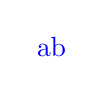
\begin{tikzpicture}
\node (n) at (0,0) [blue] {ab};\end{tikzpicture}
\newpage
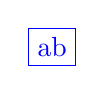
\begin{tikzpicture}
\node (n) at (0,0) [blue,draw] {ab};\end{tikzpicture}
\newpage
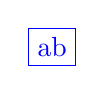
\begin{tikzpicture}
\node (n) at (0,0) [draw,blue] {ab};\end{tikzpicture}
\newpage
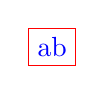
\begin{tikzpicture}
\node (n) at (0,0) [blue,draw=red] {ab};\end{tikzpicture}
\newpage
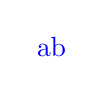
\begin{tikzpicture}
\node (n) at (0,0) [blue,fill=white] {ab};\end{tikzpicture}
\newpage
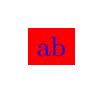
\begin{tikzpicture}
\node (n) at (0,0) [blue,fill=red] {ab};\end{tikzpicture}
\newpage

\begin{tikzpicture}
\node (n) at (0,0) [blue,fill] {ab};\end{tikzpicture}
\newpage
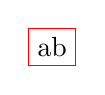
\begin{tikzpicture}
\node (n) at (0,0) [draw=red] {ab};\end{tikzpicture}
\newpage

\begin{tikzpicture}
\node (n) at (0,0) [fill=red] {ab};\end{tikzpicture}
\newpage
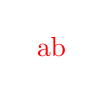
\begin{tikzpicture}
\node (n) at (0,0) [text=red] {ab};\end{tikzpicture}
\newpage
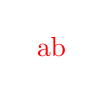
\begin{tikzpicture}
{\color{red}\node (n) at (0,0) {ab};}
\end{tikzpicture}
\newpage
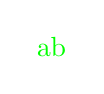
\begin{tikzpicture}
\node (n) at (0,0) [green] {ab};\end{tikzpicture}
\newpage
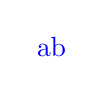
\begin{tikzpicture}
\node (n) at (0,0) [blue,rounded corners] {ab};\end{tikzpicture}
\newpage
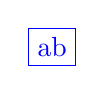
\begin{tikzpicture}
\node (n) at (0,0) [blue,draw=] {ab};\end{tikzpicture}
\newpage
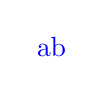
\begin{tikzpicture}
\node (n) at (0,0) [color=blue] {ab};\end{tikzpicture}
\newpage
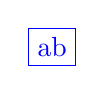
\begin{tikzpicture}
\node (n) at (0,0) [color=blue,draw] {ab};\end{tikzpicture}
\newpage
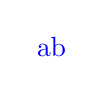
\begin{tikzpicture}
\node (n) at (0,0) [color=blue,fill=white] {ab};\end{tikzpicture}
\newpage
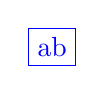
\begin{tikzpicture}
\node (n) at (0,0) [blue,draw,fill=white] {ab};\end{tikzpicture}
\newpage
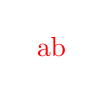
\begin{tikzpicture}
\node (n) at (0,0) [blue,text=red] {ab};\end{tikzpicture}
\newpage
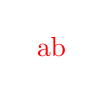
\begin{tikzpicture}
\node (n) at (0,0) [blue,fill=white,text=red] {ab};\end{tikzpicture}
\newpage

\begin{tikzpicture}
\node (n) at (0,0) [red!50] {ab};\end{tikzpicture}
\newpage

\begin{tikzpicture}
\node (n) at (0,0) [red!50,fill=white] {ab};\end{tikzpicture}
\newpage
\begin{tikzpicture}
\node (n) at (0,0) [blue,fill=white,minimum width=1cm] {ab};\end{tikzpicture}
\newpage

\begin{tikzpicture}
{\color{red}\node (n) at (0,0) [draw] {ab};}
\end{tikzpicture}
\newpage

\begin{tikzpicture}
{\color{blue}\node (n) at (0,0) [fill] {ab};}
\end{tikzpicture}
\newpage
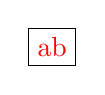
\begin{tikzpicture}
\node (n) at (0,0) [text=red,draw] {ab};\end{tikzpicture}
\newpage

\begin{tikzpicture}
\node (n) at (0,0) [text=red,fill] {ab};\end{tikzpicture}
\newpage
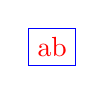
\begin{tikzpicture}
\node (n) at (0,0) [blue,text=red,draw] {ab};\end{tikzpicture}
\newpage
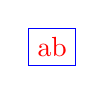
\begin{tikzpicture}
\node (n) at (0,0) [text=red,draw=blue] {ab};\end{tikzpicture}
\newpage
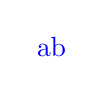
\begin{tikzpicture}
\node (n) at (0,0) [blue,draw=none] {ab};\end{tikzpicture}
\newpage
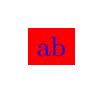
\begin{tikzpicture}
\node (n) at (0,0) [blue,fill=red,draw=none] {ab};\end{tikzpicture}
\newpage

\begin{tikzpicture}
\node (n) at (0,0) [blue,fill=] {ab};\end{tikzpicture}
\newpage
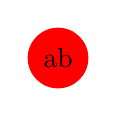
\begin{tikzpicture}
\node (n) at (0,0) [circle,fill=red] {ab};\end{tikzpicture}
\newpage

\begin{tikzpicture}
\node (n) at (0,0) [rectangle,fill=red] {ab};\end{tikzpicture}
\end{document}
